\chapter{Heat Transfer}\label{ch_Heat_Transfer}
Inside trapezoidal cavity receiver heat transfer takes place via convection (conduction and advection) and radiation. Since air is present inside trapezoidal cavity receiver, it will lead to convection given temperature difference. Apart from that Top, left and right walls of the cavity, bottom glass cover and pipes will be exchanging heat via radiation. Temperature gradient inside the trapezoidal cavity receiver will lead to convection. However possibility of convection is depends on the relative direction of the temperature gradient with respect to the gravity.  Consider two vectors, first representing the direction of temperature gradient and second representing direction of gravity. When first vector is in the direction of second vector, maximum amount of convection takes place as due to density difference hot water will float and it will have tendency of moving opposite of the direction of gravity while colder air will have a tendency to move in the direction of gravity. This phenomena will continue until temperature gradient vector is completely opposite of the gravity. Which is the scenario in our study. Experiments done on the trapezoidal cavity receiver shows that top wall of the cavity is at higher temperature relative to the bottom glass temperature. In this case temperature gradient vector is opposite to the gravity so, convection should not occur. However, since there are other parts like pipes through which working fluid is passing through temperature gradient exists in lateral direction as well. But experiments and simulations performed on trapezoidal cavity receiver shows that these temperature gradient are quite smaller than the temperature gradient existing between top wall and the bottom glass. Thus even though some local convective currents do form. Its contribution in the overall heat transfer is very low. Mohan et. al.\citep{MOHAN201837} has shown that contribution of advection in the convection inside trapezoidal cavity receiver is very low. To show that two simulations were performed by him. Inside trapezoidal cavity receiver, heat transfer was modeled with convection (conduction and advection) in one case while in another case it was modeled with conduction alone. Result shows less than 1 \% of difference in the Nusselt number at the hot wall obtained in both the simulations. Keeping that in mind, in the present work heat transfer has been modeled with conduction only and advection has been ignored. To verify the conduction model same problem is solved here as has been by Mohan et. al.\citep{MOHAN201837} and its result has been compared against theirs. After that taking another step forward, radiation has been added in the model and results obtained by this new conduction and radiation model has been compared against Mohan et. al.\citep{MOHAN201837} work. 


\section{Validation of conduction model}\label{sec:validationConduction}
For validation purpose conduction model used for present study is tested against the benchmark solution. In this case benchmark solution is taken to be Mohan et. al.\citep{MOHAN201837} work.
\subsection{Problem Statement}
For verification of the conduction model, a trapezoidal cavity has been considered which is shown in the fig. \ref{geometry_modified}. Top wall of the cavity is kept at constant temperature of 623 K. Left and right cavity walls are insulated. Heat transfer coefficient of 25 W/$m^2$ is defined for convection with the ambient which is kept at the temperature of 300 K. Bottom width of the cavity is 0.5 m and depth is 0.1 m.

\begin{figure}[H]
\begin{center}
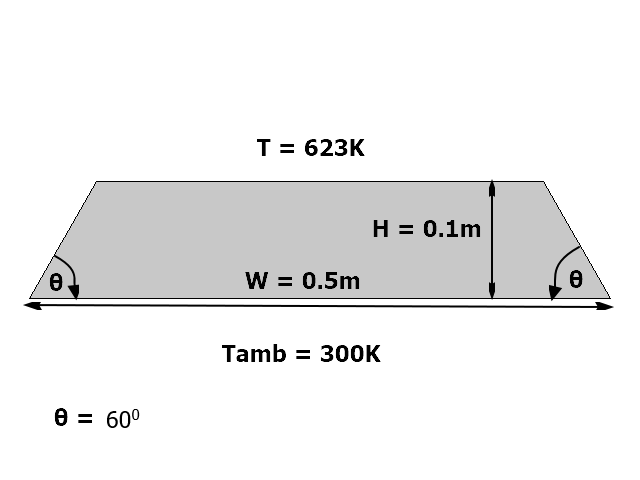
\includegraphics[width = 0.9\textwidth]{geometry_modified.png}
\caption{Trapezoidal cavity geometry}
\label{geometry_modified}
\end{center}
\end{figure}
\subsection{Grid independence testing}
Meshing has been done using free triangular elements. For grid independence testing	maximum allowed element-size was varied and variation in Nusselt number at the hot wall was observed which can be seen in the table \ref{gridTestCond}. 


\begin{table}[H]
\centering
\caption{Grid independence test result for conduction}
\label{gridTestCond}
\begin{tabular}{@{}|c|c|@{}}
\toprule
\textbf{Maximum Element Size (m)} & \textbf{Nusselt Number} \\ \midrule
0.1650                             & 1.103                  \\ \midrule
0.1000                            & 1.099                  \\ \midrule
0.0650                            & 1.097                  \\ \midrule
0.0500                            & 1.096                  \\ \midrule
0.0335                            & 1.096                  \\ \bottomrule
\end{tabular}
\end{table}

It is quite apparent from the table \ref{gridTestCond} that variation in Nusselt number is ceased after maximum element size of 0.05 m. So finally simulation was performed using this element size.

\subsection{Result comparison}
Nusselt Number at the hot wall and total heat provided by hot wall to the rest of the cavity has been compared in the table \ref{tab:conductionModelResultValidation}.

\begin{table}[H]
\centering
\caption{Conduction model result validation}
\label{tab:conductionModelResultValidation}
\begin{tabular}{@{}|c|c|c|@{}}
\toprule
\textit{\textbf{At the hot wall}} & \textbf{Present Work} & \textbf{Benchmark} \\ \midrule
Total heat (W)                    & 50.35                 & 49.00              \\ \midrule
Nusselt number                    & 1.10                  & 1.10               \\ \bottomrule
\end{tabular}
\end{table}

Temperature distribution along the vertical axis of cavity has been show in the fig. \ref{fig:validationConduction}

% \begin{figure}
% \centering
% \begin{minipage}{\textwidth}
%   \centering
%   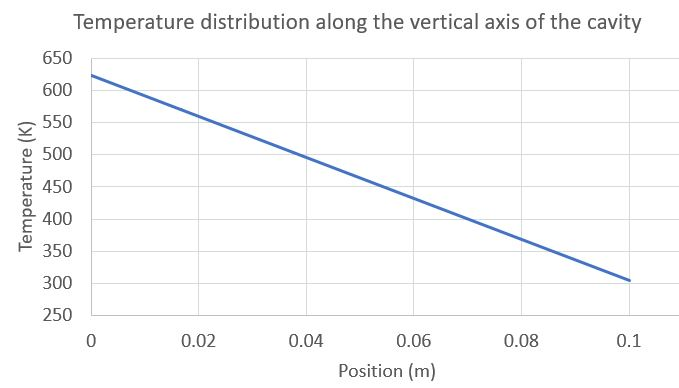
\includegraphics[width=\linewidth]{TrapezoidalCavityConductionTemperatureVerticalAxis.JPG}
%   \caption{figure}{A figure}
%   \label{fig:test1}
% \end{minipage}%
% \begin{minipage}{\textwidth}
%   \centering
%   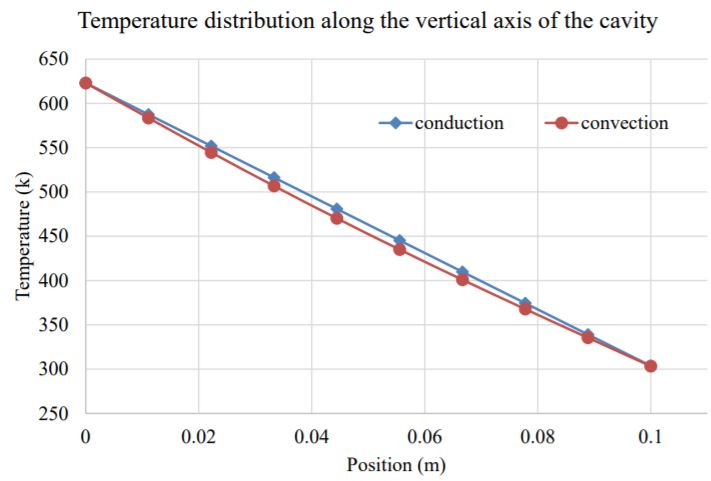
\includegraphics[width=\linewidth]{SarathTrapezoidalCavityConductionTemperatureVerticalAxis.JPG}
%   \caption{figure}{Another figure}
%   \label{fig:test2}
% \end{minipage}
% \end{figure}

\begin{figure}[H]
\centering     %%% not \center
\subfigure[Present work]{\label{fig:a}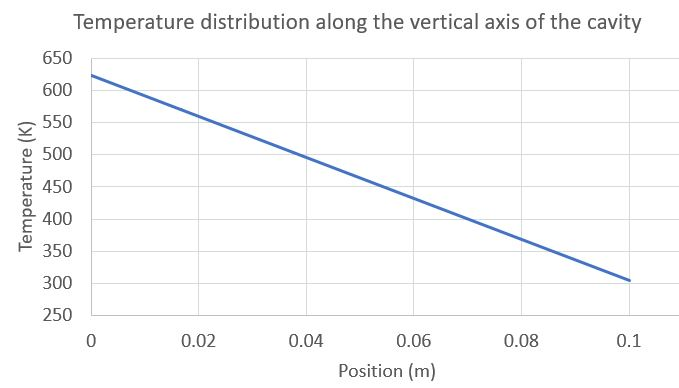
\includegraphics[width=120mm]{TrapezoidalCavityConductionTemperatureVerticalAxis.JPG}}
\subfigure[Benchmark\citep{MOHAN201837}]{\label{fig:b}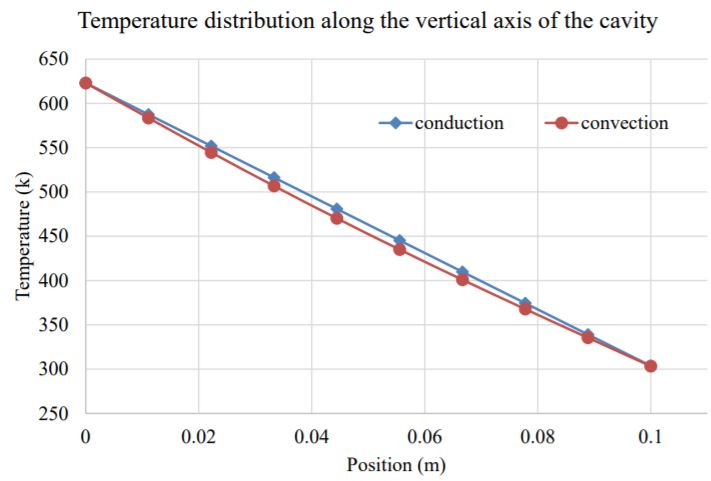
\includegraphics[width=120mm]{SarathTrapezoidalCavityConductionTemperatureVerticalAxis.JPG}}
\caption{Comparison of temperature variation for conduction validation}
\label{fig:validationConduction}
\end{figure}

\subsection{Conclusion}

From table \ref{tab:conductionModelResultValidation} it can be seen that values of Nusselt number and heat provided by the hot wall to the rest of the cavity as calculated by present work's conduction model matches quite closely to the benchmark results. And from fig. \ref{fig:validationConduction} it can be seen that temperature profile along vertical axis of the cavity as calculated by present work's conduction model is similar to the the benchmark result. Thus it is concluded that conduction model of present work agrees quite well with the benchmark.

%%%%%%%%%%%%%%%%%%%%%%%%%%%%%%%%%%%%%%%%%%%%%%%%%%%%%%%%%%%%%%%%%%%%%%%%%%%%%
%%%%%%%%%%%%%%%%%%%%%%%%%%%%%%%%%%%%%%%%%%%%%%%%%%%%%%%%%%%%%%%%%%%%%%%%%%%%%
%%%%%%%%%%%%%%%%%%%%%%%%%%%%%%%%%%%%%%%%%%%%%%%%%%%%%%%%%%%%%%%%%%%%%%%%%%%%%

\section{Validation of conduction+radiation model}
In the next step radiation is added in the conduction model to account for heat transfer in trapezoidal cavity receiver. For validation purpose conduction+radiation model used for present study is tested against the benchmark solution. In this case benchmark solution is taken to be Mohan et. al.\citep{MOHAN201837} work.
\subsection{Problem Statement}
For verification of the conduction+radiation model, problem statement of the section \ref{sec:validationConduction} has been used with added modification. Emissivity of top wall was taken to be 0.3, for side walls it was taken to be .05 and for bottom glass it was 0.9. 
\begin{figure}[H]
\begin{center}
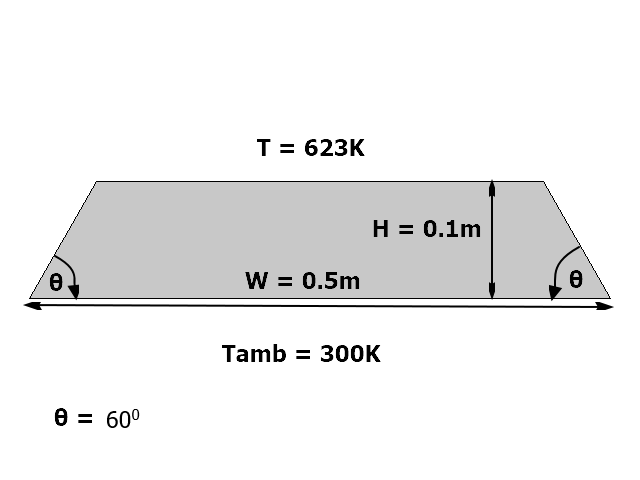
\includegraphics[width = 0.9\textwidth]{geometry_modified.png}
\caption{Trapezoidal cavity geometry}
\label{geometry_modified}
\end{center}
\end{figure}

For radiation modeling surface to surface model has been used. Radiation group was defined to account for internal radiation which includes top, left and right walls along with the glass bottom. Apart from that radiation to environment was defined from glass as well.
\subsection{Grid independence testing}
Meshing has been done using free triangular elements. For grid independence testing	maximum allowed element-size was varied and variation in Nusselt number at the hot wall was observed which can be seen in the table \ref{gridTestCond}. 


\begin{table}[H]
\centering
\caption{Grid independence test result for conduction}
\label{gridTestCond}
\begin{tabular}{@{}|c|c|@{}}
\toprule
\textbf{Maximum Element Size (m)} & \textbf{Nusselt Number} \\ \midrule
0.1650                            & 19.687                  \\ \midrule
0.1000                            & 19.682                  \\ \midrule
0.0650                            & 19.633                  \\ \midrule
0.0500                            & 19.626                  \\ \midrule
0.0335                            & 19.622                  \\ \midrule
0.0265                            & 19.619                  \\ \midrule
0.0185                            & 19.618                  \\ \midrule
0.0100                            & 19.617                  \\ \midrule
0.0050                            & 19.617                  \\ \bottomrule
\end{tabular}
\end{table}

It is quite apparent from the table \ref{gridTestCond} that variation in Nusselt number ceased after maximum element size of 0.01 m. So finally simulation was performed using this element size.

\subsection{Result comparison}
Nusselt Number at the hot wall, total heat provided by hot wall to the rest of the cavity via radiation and total heat provided by hot wall to the rest of the cavity has been compared in the table \ref{tab:conductionRadiationModelResultValidation}.

\begin{table}[H]
\centering
\caption{Conduction+radiation model result validation}
\label{tab:conductionRadiationModelResultValidation}
\begin{tabular}{@{}|c|c|c|@{}}
\toprule
\textit{\textbf{At the hot wall}} & \textbf{Present Work} & \textbf{Benchmark} \\ \midrule
Total heat (W)                    & 895.98                & 899.90             \\ \midrule
Total radiative heat (W)          & 840.63                & 846.99             \\ \midrule
Nusselt number                    & 19.62                 & 20.07              \\ \bottomrule
\end{tabular}
\end{table}

Temperature distribution along the vertical axis of cavity has been show in the fig. \ref{fig:validationConductionRadiation}

\begin{figure}[H]
\centering     %%% not \center
\subfigure[Present work]{\label{fig:a}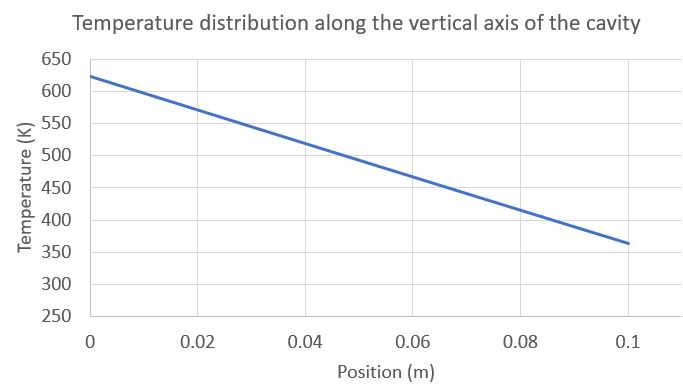
\includegraphics[width=120mm]{TrapezoidalCavityConductionRadiationTemperatureVerticalAxis.JPG}}
\subfigure[Benchmark\citep{MOHAN201837}]{\label{fig:b}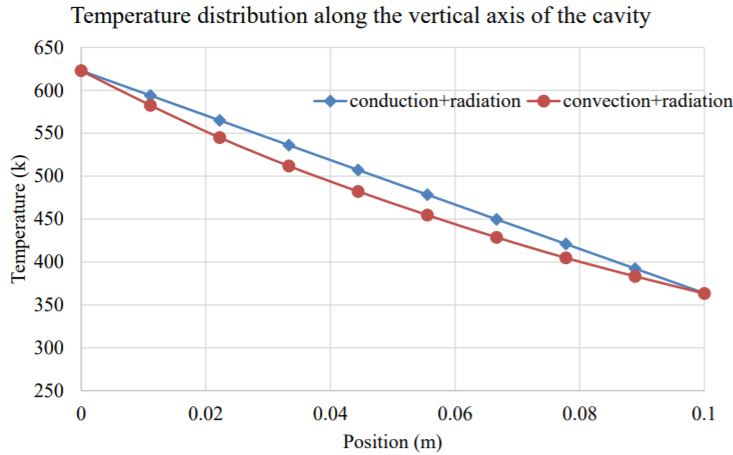
\includegraphics[width=120mm]{SarathTrapezoidalCavityConductionRadiationTemperatureVerticalAxis.JPG}}
\caption{Comparison of temperature variation for conduction validation}
\label{fig:validationConductionRadiation}
\end{figure}

\begin{figure}[H]
\centering     %%% not \center
\subfigure[Present work]{\label{fig:a}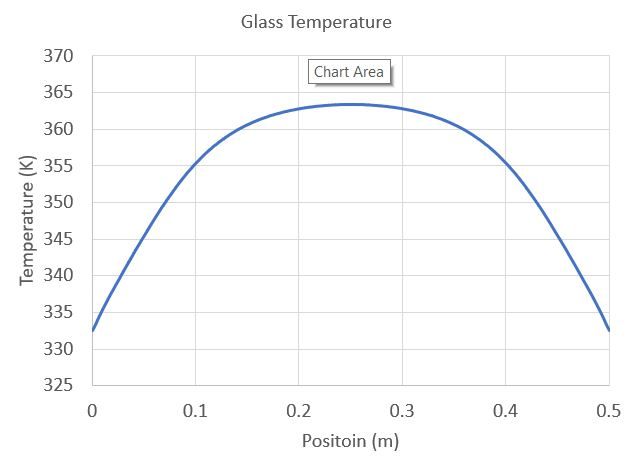
\includegraphics[width=120mm]{GlassTemperatureValidation.JPG}}
\subfigure[Benchmark\citep{MOHAN201837}]{\label{fig:b}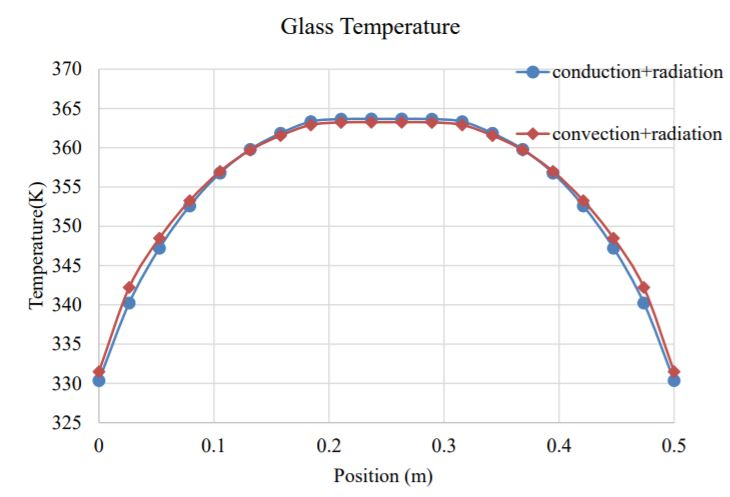
\includegraphics[width=120mm]{SarathGlassTemperatureValidation.JPG}}
\caption{Comparison of temperature variation for conduction validation}
\label{fig:validationConductionRadiationGlass}
\end{figure}

\subsection{Conclusion}

From table \ref{tab:conductionRadiationModelResultValidation} it can be seen that values of Nusselt number and heat provided by the hot wall to the rest of the cavity via radiation and conduction as calculated by present work's conduction model matches quite closely to the benchmark results. And from fig. \ref{fig:validationConductionRadiation} and \ref{fig:validationConductionRadiationGlass} it can be seen that temperature profile along vertical axis of the cavity and glass temperature as calculated by present work's conduction model is similar to the the benchmark result. Thus it is concluded that conduction+radiation model or heat transfer model of present work agrees quite well with the benchmark.

This concludes validation part of the heat transfer model. Now in further section the same model will be provided heat flux data as calculated from ray optics simulation to obtain overall loss from the cavity.

\section{Heat loss analysis in trapezoidal cavity receiver}
Heat loss analysis for TCR has been performed using combined conduction and radiation model in COMSOL Multiphysics 5.1 which will be explored in this section. Result of ray optics simulation has been used as input for heat transfer simulation. Heat received by different surfaces inside TCR as calculated in chapter \ref{ch:RayOps} is used here for loss study in TCR.

\subsection{Problem Statement}
A trapezoidal cavity receiver contains 8 pipes which carry water as working fluid. Top, left and right sides of the cavity are well insulated while bottom glass surface is engaged in convection and radiation with the environment. All the surfaces inside the TCR are involved in internal radiation with each other. Specification of the TCR can be seen in table \ref{tab:tcrspectab}. Geometry of TCR as created in COMSOL Multiphysics 5.1 has been show in the fig. \ref{fig:tcrgeo}.

\begin{table}[H]
\centering
\caption{TCR specification}
\label{tab:tcrspectab}
\begin{tabular}{@{}|l|c|@{}}
\toprule
\textbf{Items}                      & \textbf{Dimensions} \\ \midrule
Bottom width of the cavity          & 500 mm              \\ \midrule
Top width of the cavity             & 300 mm              \\ \midrule
Side length of the cavity           & 141 mm              \\ \midrule
Depth of the cavity                 & 100 mm              \\ \midrule
No of tubes in the cavity           & 8                   \\ \midrule
Absorber tube inner diameter        & 26.7 mm             \\ \midrule
Absorber tube outer diameter        & 33.4 mm             \\ \midrule
Absorber length                     & 384 m               \\ \bottomrule
\end{tabular}
\end{table}

\begin{figure}[H]
\begin{center}
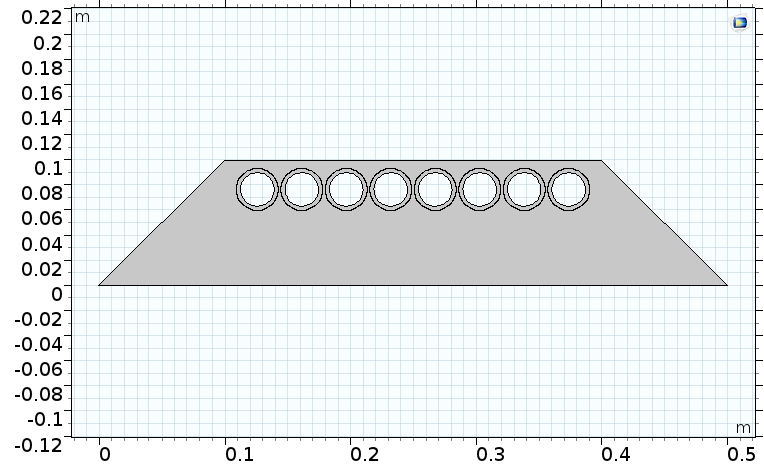
\includegraphics[width = 0.9\textwidth]{geometry.png}
\caption{Trapezoidal cavity receiver geometry}
\label{fig:tcrgeo}
\end{center}
\end{figure}


When TCR are used for industrial purposes gap between pipes carrying the working fluid is almost negligible as they expand due to heat. To imitate that here pipes are separated from each other by just 1 mm of distance. Pipes are kept very close to the top surface of the cavity to avert the possibility of formation of convective currents. Keeping that in mind distance between top surface of the cavity and circumference of pipes is kept to be 7 mm. 


\subsection{Modeling}
Heat transfer in the cavity is modeled using conduction and radiation method. For radiation surface to surface approach has been taken using hemicube method. Radiation resolution for hemicube method is kept to be 256 after resolution independence test.

\subsection{Grid Independence test}
Free triangular elements have been selected for meshing the geometry. 
















